\subsection{Unregelmäßigkeiten in der Klassifikation des Portals "`Babw"'}
    \label{section:findingsTeachersAbnormalitiesBabw}
    Dieses Kapitel stellt die Auffälligkeiten in der Klassifikation
    der Seite der Lehrenden und Betreuenden im Studienportal
    "`B.A. Bildungswissenschaft"' vor.
    Zusätzlich erfolgt eine Erklärung,
    wodurch die jeweilige Unregelmäßigkeit begründet ist.

    \paragraph{Zwei Mitarbeiter ohne Lehrgebiet}
    Die Klassifikation enthält für zwei Mitarbeiter kein Lehrgebiet.
    Im ersten Fall nennt die Webseite kein Lehrgebiet,
    weshalb die Klassifikation an dieser Stelle korrekt ist.
    Der zweite Kontakt ist ein Mitarbeiter einer fremden Universität,
    weshalb dessen Lehrgebiet kein Verweis auf eine andere Seite,
    sondern einfacher Text ist.
    Der verwendete Selektor "`div.team-member-des > p > a:first-child"'
    hat diesen Text nicht erfasst, da er einen Link sucht.

    \paragraph{Unvollständige Namen zweier Mitarbeiter}
    Zwei Kontakte besitzen laut Klassifikation den Namen "`Prof."' bzw. "`Dr."'.
    In diesen Fällen stehen Titel und Name in getrennten strong-Elementen.
    Da der Name eines Mitarbeiters ein skalares Feature ist,
    wurde nur das erste Element vom System erfasst.

    \paragraph{Falsche und fehlende Hervorhebungen durch Annotationen}
    Einige Elemente der Seite wurden durch das Annotator inkorrekt oder nicht hervorgehoben.
    Aus Abbildung \ref{image:findingTeachersAnnotationsOverview} geht bereits hervor,
    dass Bilder hiervon betroffen sind und Annotator diese markiert.
    Abbildung \ref{image:findingTeachersBaBwWrongAnnotations}
    veranschaulicht, dass Telefonnummern und Raumangaben oftmals verschoben annotiert werden.
    Der Grund ist die in Kapitel \ref{section:solutionDetailsClassificationServiceClassification}
    beschriebene Konflikt bei der Bestimmung eines eindeutigen Selektor.
    Allerdings ist auch zu beobachten, dass einige Angaben,
    wie die E-Mail-Adresse in Abbildung \ref{image:findingTeachersBaBwWrongAnnotations}
    überhaupt nicht markiert werden.

    \begin{figure}[htb]
        \centering
        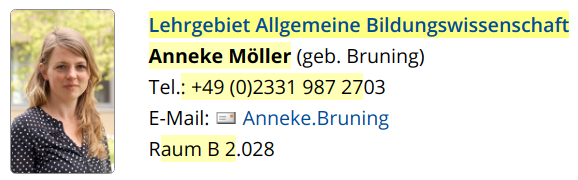
\includegraphics[width=0.5\textwidth]{../resources/findings/case-study-1/babw/annotations/missing-annotation.png}
        \caption{Fehlerhafte Hervorhebung durch Annotationen}
        \label{image:findingTeachersBaBwWrongAnnotations}
    \end{figure}
